%%
%% Copyright (c) 2018-2019 Weitian LI <liweitianux@sjtu.edu.cn>
%% Creative Commons BY 4.0
%%

\chapter{再电离时期的探测}
\label{chap:detection}


\emph{\acf{eor}}是早期宇宙的一段缺乏了解的时期,目前的理论研究以及有限的观测证据表明
该时期从宇宙大爆炸之后约 \SI{300}{\Myr} 持续到约 \SI{1}{\Gyr},对应红移范围
约为 \numrange{6}{15} (参见 \citeay{koopmans2015} 及其所引文献).
充分探明并理解该时期是为进一步揭示更早的\ac{cd}和\ac{da}($z > 15$)、
建立完整的宇宙演化图景的关键环节.
在低频射电波段(约 \SIrange{50}{200}{\MHz})
探测源自再电离时期的 21\,cm 信号(即\emph{EoR 信号})
是目前研究该时期的最直接而有效的办法 \cite{madau1997,tozzi2000,furlanetto2006}.


%=====================================================================
\section{EoR 信号}
\label{sec:eor-signal}

%---------------------------------------------------------------------
\subsection{21\texorpdfstring{\,}{ }cm~谱线}

中性氢的 21\,cm 谱线
首次由 Hendrik Christoffel van de Hulst 在 1945 年提出 \cite{vanDeHulst1945},
并由 Harold Ewen 和 Ed Purcell 在 1951 年观测到 \cite{ewen1951}.

简并度 (degeneracy factor)
固有距离 (proper distance)
出射亮度 (emergent brightness)
视亮度 (apparent brightness)

physical theory ...
EoR observation principle ...
delta-Tb (spin temperature) ...


%---------------------------------------------------------------------
\subsection{亮温度}

21 cm 信号平均强度随红移和频率(亦即宇宙年龄)的变化规律.
在最初的宇宙黑暗时期,重子物质与 CMB 光子脱耦并随宇宙膨胀而冷却,结构也开始形成,
其中的冷气体可通过 21 cm 吸收信号被观测;
然后第一代恒星及星系产生并辐射大量 Lyα 光子,
使得中性氢的自旋态与气体温度紧密耦合,导致强烈的 21 cm 吸收信号;
但随着星系的大量形成而加热其中的气体,中性氢的 21 cm 辐射信号逐渐变强;
最后中性氢被逐步电离完,21 cm 辐射信号也衰减至消失
\cite{pritchard2012}.


%=====================================================================
\section{探测方法}
\label{sec:det-methods}

目前有三种测量 EoR 信号的方法,由易到难分别为:
(1) 测量全天总功率;
(2) 测量功率谱;
(3) 直接获取再电离区域的图像.

第一种方法仅测量 EoR 信号的全天总功率随红移(即观测频率)的变化,
所得结果可以用于推断物质的电离过程,帮助检验和约束再电离模型
\cite{pritchard2012,liu2016}.
该方法相对简单易行,通常采用小型专用设备,一般包含单个或少量天线.
目前已有一批采用该方法的 EoR 探测实验,主要包括
位于澳大利亚的 \ac{edges} \cite{bowman2008} 和
\ac{bighorns} \cite{sokolowski2015}、
位于美国的 \ac{leda} \cite{greenhill2012}、
位于墨西哥的 \ac{sci-hi} \cite{voytek2014}
以及位于印度的 \ac{saras} \cite{singh2018}.
值得一提的是,\acs{edges} 在 2018 年初报导称发现全天平均射电信号在 \SI{78}{\MHz}
附近存在吸收,该吸收信号所处位置大致符合早期恒星所引发的 21\,cm 信号,
但其强度是目前理论预测值的两倍以上 \cite{bowman2018}.

后两种方法则进一步测量 EoR 信号的统计分布规律甚至三维图像,能够提供更加全面丰富
的信息用于系统性地研究\acl{eor}.
尽管这两种测量方法更加强大有效,但需要大型低频干涉阵列,
如 \autoref{sec:instruments} 所介绍的主要干涉阵列,
其中仅有 \acs{ska} 将拥有足够高的灵敏度实现对再电离区域的直接成像观测.


%=====================================================================
\section{主要困难}
\label{sec:det-difficulties}

EoR 探测实验,尤其是采用干涉阵列,面临着一系列困难.
这些困难可主要分为以下几类:
\begin{itemize}
\item
\emph{前景干扰:}
源自银河系以及河外源的前景辐射非常强烈,可达数百 \si{\kelvin},
是 EoR 信号(仅约几 \si{\mK} 至几十 \si{\mK})的 \numrange{4}{5} 个数量级.
虽然对干涉阵列而言重要的是辐射的空间涨落幅度而非其平均强度,
但是前景辐射的涨落幅度仍达数 \si{\kelvin} 到数十 \si{\kelvin},
远远压制了待测 EoR 信号 \cite{zaroubi2013}.
\autoref{fig:eor-foregrounds} 显示了主要的前景成分及其在
\SI{120}{\MHz} 处的强度.
因此,即便是轻微的前景处理不当,都会导致微弱的 EoR 信号被淹没而无法被捕捉到.
此外,部分前景成分(如银河系\ac{rad-syn})存在显著偏振,
该偏振成分可能发生泄漏而影响前景强度的测量,即\ac{pl}效应 (ref???),
导致前景的频谱结构复杂化而变得更加难以处理 (ref???).
如何处理强烈的前景干扰并成功分离 EoR 信号,
是目前 EoR 探测领域的一个关键任务,
不仅需要系统深入地理解前景的特征 \cite{offringa2016,carroll2016,procopio2017} (ref???),
还需要研发有效的前景扣除与信号分离算法 \cite{chapman2015,chapman2016} (ref???).

\begin{figure}[tbp]
  \centering
  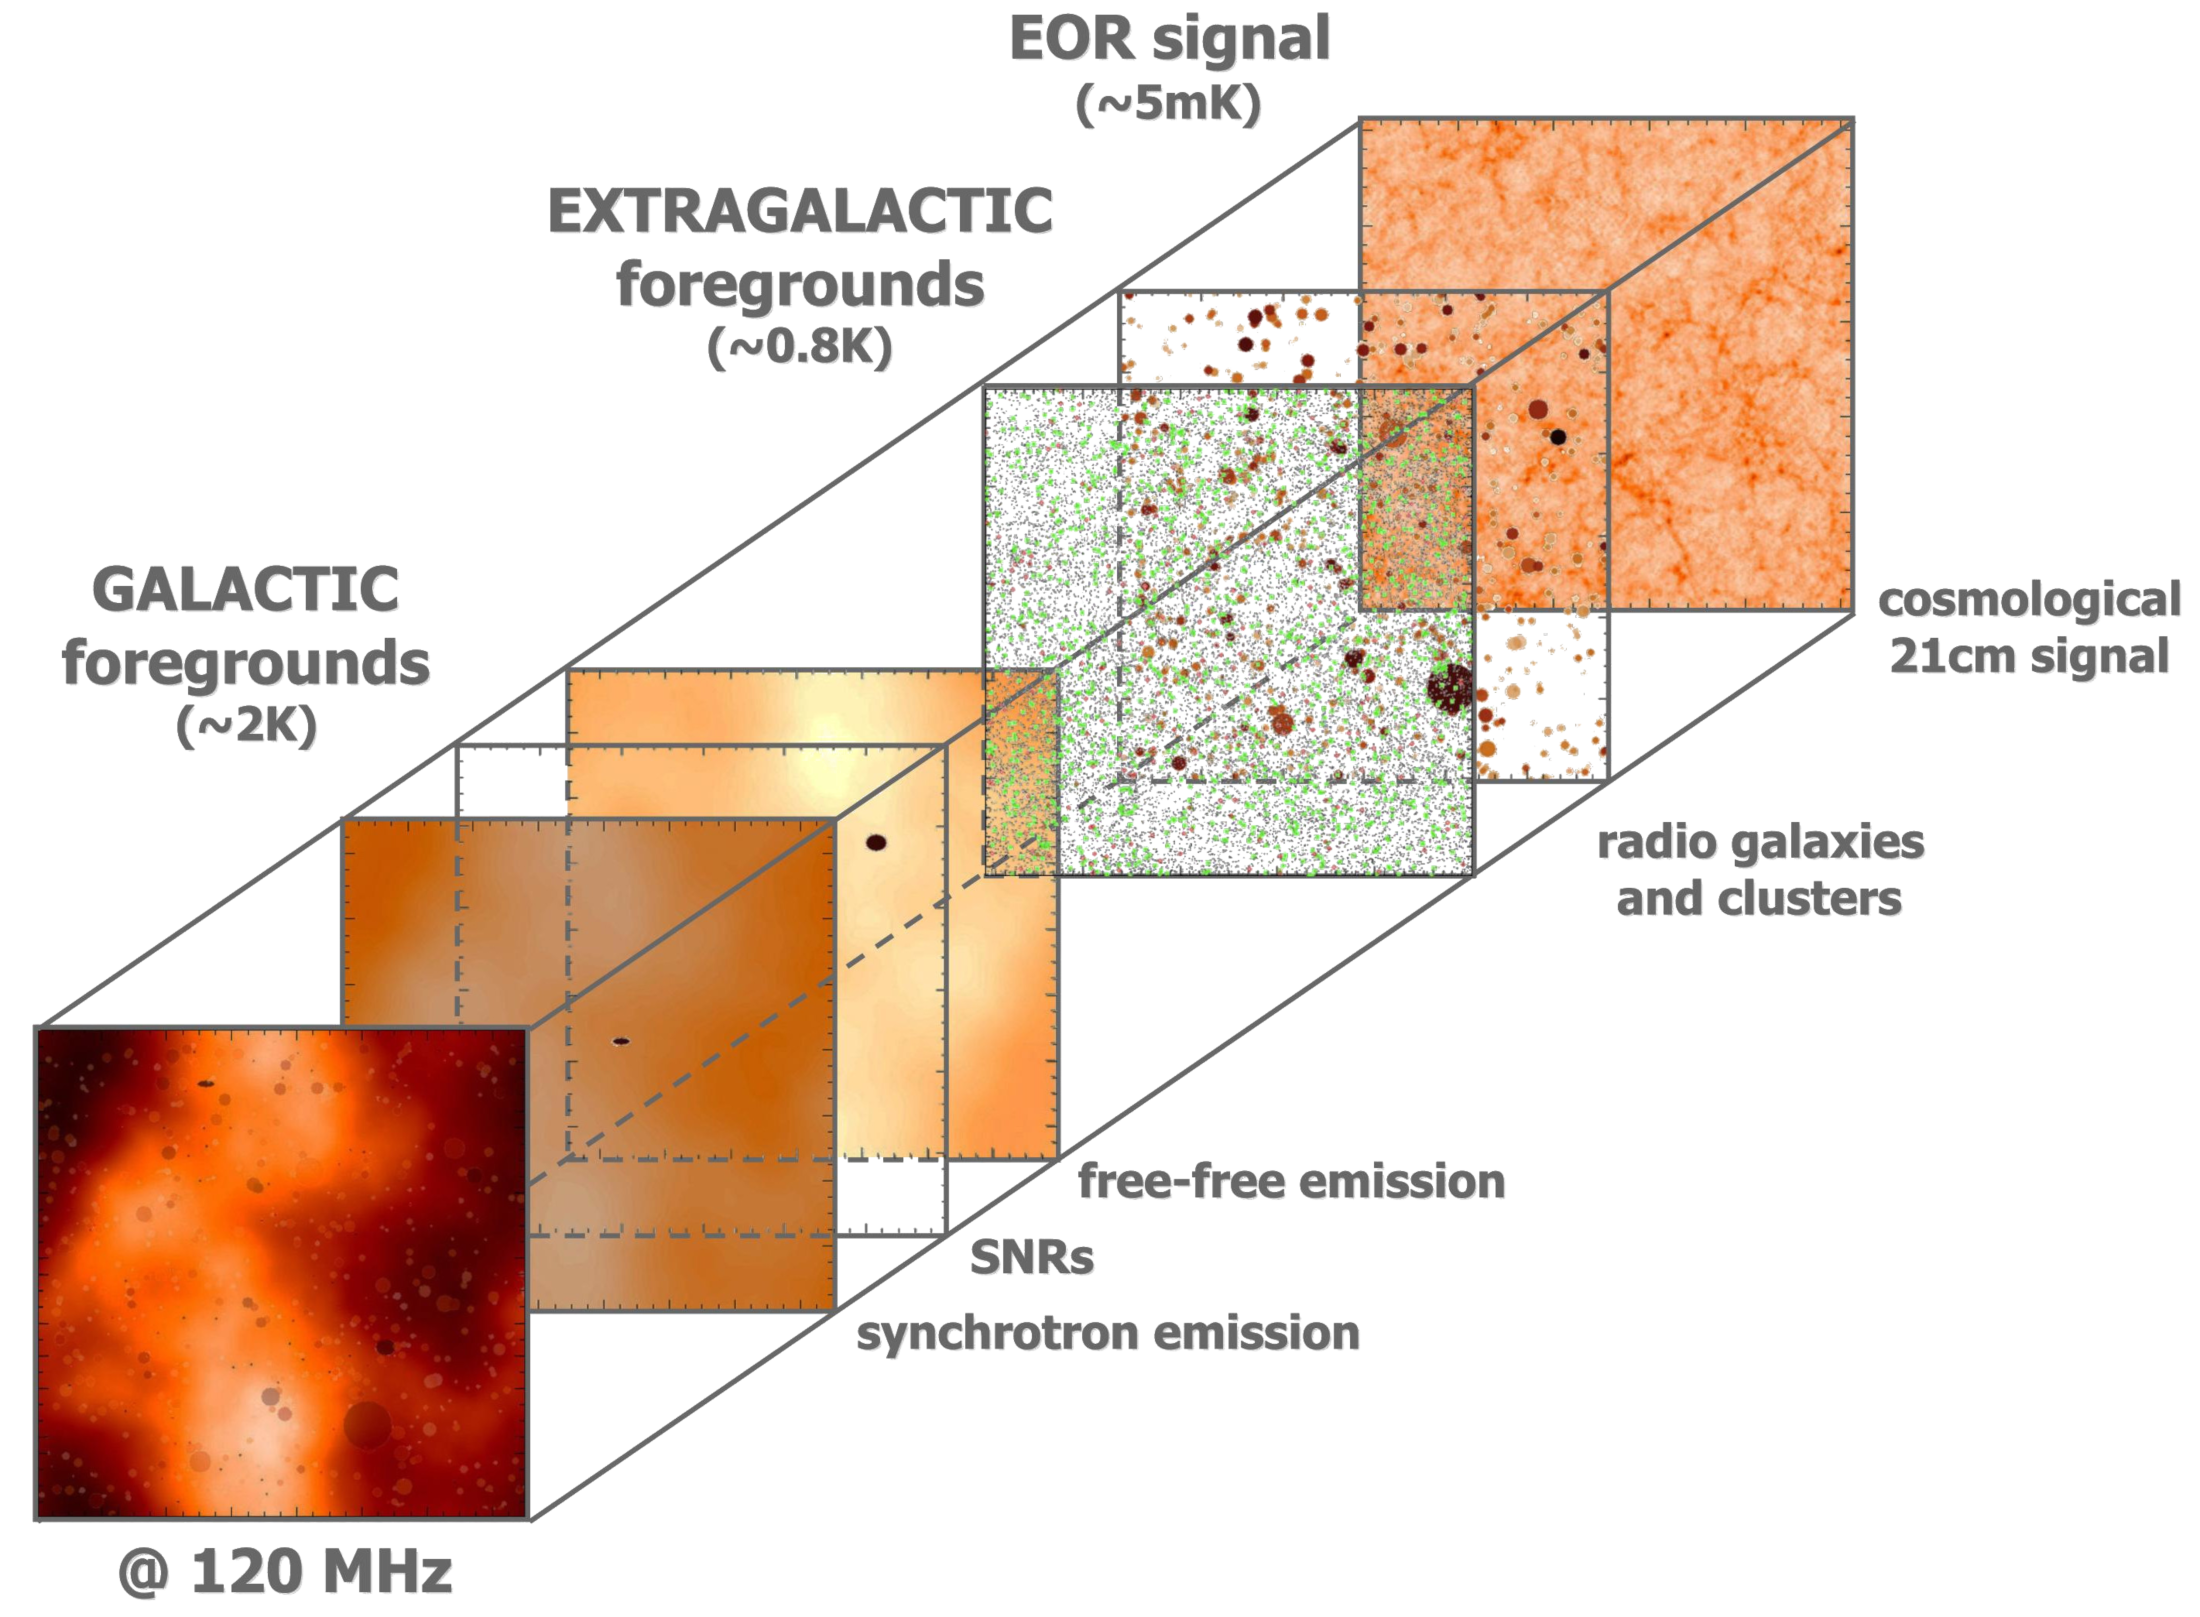
\includegraphics[width=0.7\textwidth]{eor-foregrounds}
  \bicaption[主要前景成分及其强度示意图]{%
    主要前景成分以及强度示意图.
    图中的数值代表在 \SI{120}{\MHz} 处的\acuse{rms}\acl{rms}值.
  }{%
    A diagram showing the major foreground components contaminating
    the EoR signal.
    The numbers in the figure represent the \acs{rms} values
    at \SI{120}{\MHz}.
    \\\textcopyright{}
    \citeay{zaroubi2013}.
  }
  \label{fig:eor-foregrounds}
\end{figure}

%.......................................
\item
\emph{人工源的\acl{rfi}:}
随着科技的进步和社会的发展,人类活动产生的无线电波已在地球上无处不在,
对射电天文观测产生了严重的\acf{rfi}.
这些人工源主要有:\ac{am}和\ac{fm}广播、卫星通信、\ac{gps}信号、
对讲机、手机、移动通信基站、航空通信、雷达、等等.
虽然 EoR 探测设备通常建设在人烟稀少的射电宁静区域,但是仍不可避免受到
人工源的 \ac{rfi},甚至由月亮以及太空碎片反射回来的无线电波都可能
对 EoR 观测产生一定程度的影响 \cite{mckinley2013,tingay2013rfi}.
如\autoref{fig:rfi-mwa} 所示的是 MWA 在其各子频段的\ac{vis}数据
被标记为 \ac{rfi} 的比例,其中突显了\ac{fm}广播、卫星通信以及数字电视
等干扰源对 EoR 探测所造成的影响.
\ac{rfi} 的强度通常会高出天空信号的若干个数量级 \cite{bentum2011} (ref???),
并且实时发生变化.
目前的主要办法是识别并屏蔽存在明显 \ac{rfi} 的时间和频率片段
\cite{offringa2010,offringa2012,prasad2012},
但是残留的干扰可能会对前景处理以及 EoR 信号测量均产生严重影响 \cite{offringa2015}.

\begin{figure}[tbp]
  \centering
  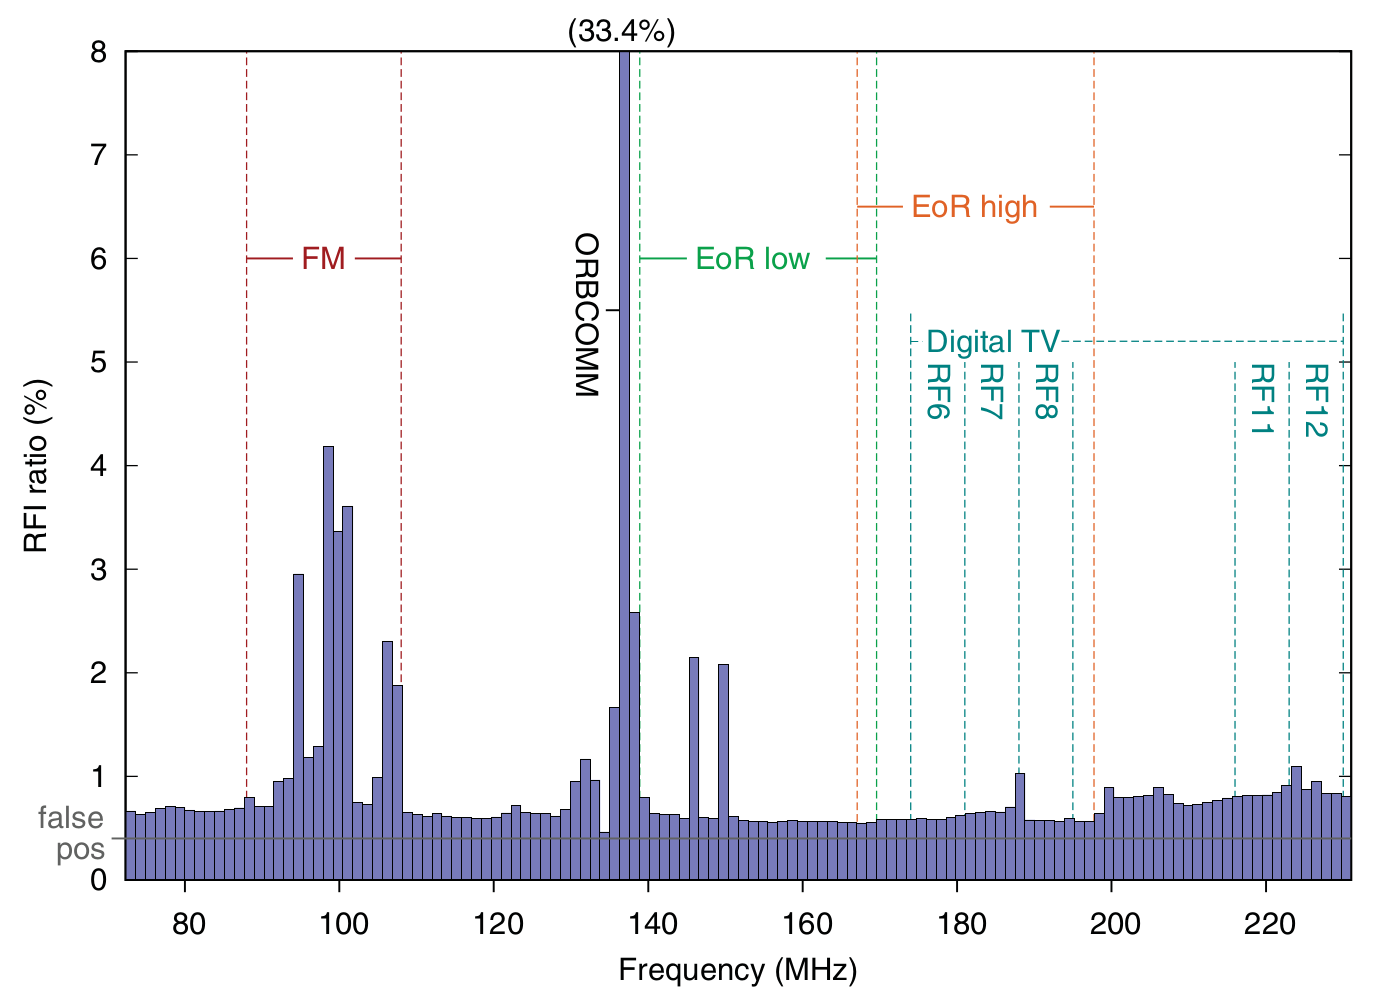
\includegraphics[width=0.7\textwidth]{RFI-MWA}
  \bicaption[MWA 各子频段内的 RFI 比例]{%
    MWA 各子频段的\acs*{vis}数据被标记为 \acs*{rfi} 的比例.
  }{%
    The \acs*{rfi} occupancy, calculated as the percentage of
    visibilities that are detected as \acs*{rfi} by the flagger,
    per sub-band for the MWA.
    \\\textcopyright{}
    \citeay{offringa2015}.
  }
  \label{fig:rfi-mwa}
\end{figure}

%.......................................
\item
\emph{电离层干扰:}
\acf{ionosphere}是地球大气层上部被太阳辐射电离的部分,从约 \SI{60}{\km}
延伸至约 \SI{1000}{\km} 的高空,覆盖了大气层的\ac{thermosphere}以及
部分\ac{mesosphere}和\ac{exosphere},是地球\ac{magnetosphere}的内界
(如\autoref{fig:ionosphere} 所示).
电离层的大气已经非常稀薄,因此被太阳辐射中的紫外线和 X 射线电离的
空气分子所产生的自由电子在复合前可以短暂地自由活动,形成等离子体,能够对电磁波的
传播产生影响.
在 \SI{300}{\MHz} 的低频波段,电离层主要对电磁波产生折射、
传播延迟、Faraday 旋转等影响,导致测量数据存在相位和幅度误差
\cite{intema2009,thompson2017}.
由于主要受太阳活动的影响,电离层的状态会随时间和位置而发生剧烈变化,
因此对干涉阵列各天线产生的干扰程度也存在差异且时刻发生变化.
为了高质量的图像,必须实时(分钟量级???)校准观测数据 (ref???),
而且对每个天线施加的校准需要有针对性 (ref???),这将成为一个严重的计算负担,
还需要发展更加有效的电离层校准算法 \cite{intema2009,deGasperin2018}.

\begin{figure}[tbp]
  \centering
  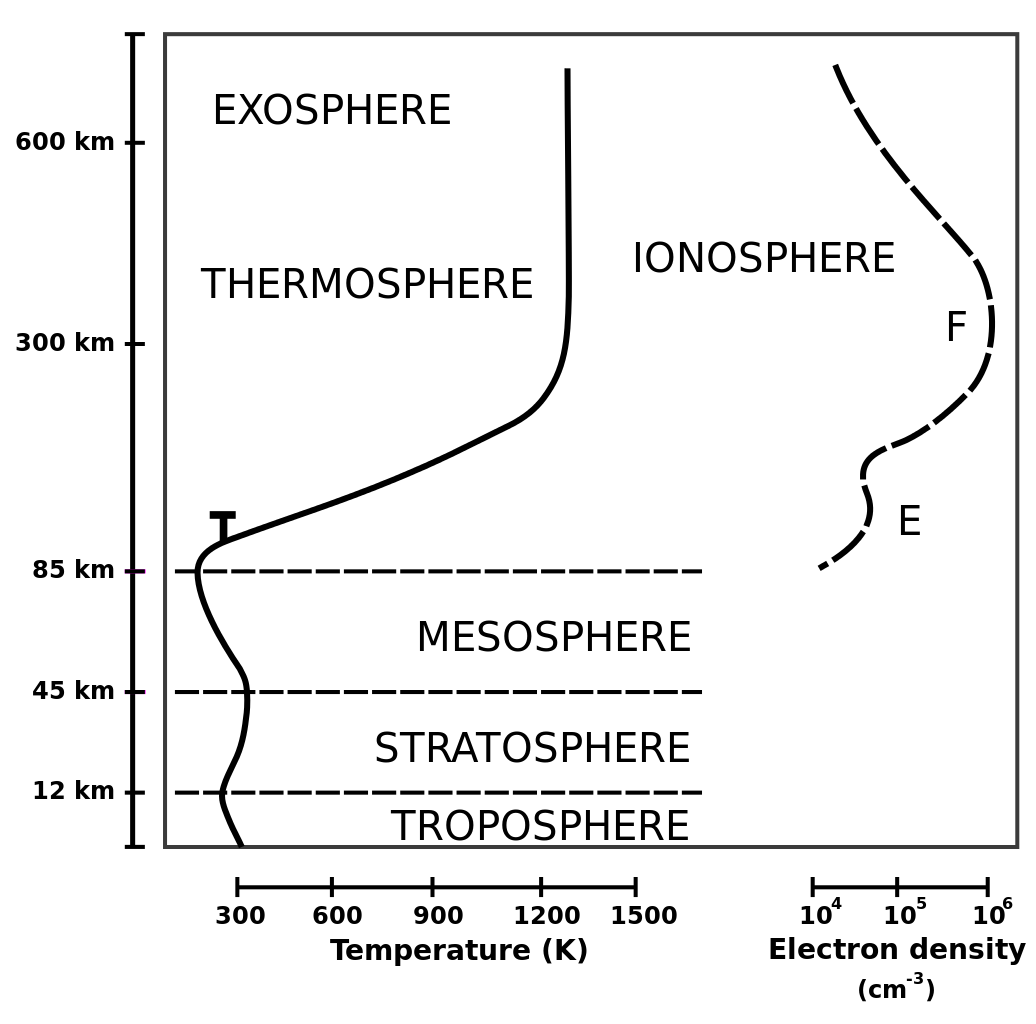
\includegraphics[width=0.5\textwidth]{atmosphere-with-ionosphere}
  \bicaption[大气层和电离层的关系]{%
    地球的大气层和电离层之间的关系.
    电离层是大气层上部被太阳辐射电离的部分.
  }{%
    The relation between Earth's atmosphere and ionosphere, which
    is the ionized part of upper atmosphere.
    \\\textcopyright{}
    Bhamer,
    \url{https://en.wikipedia.org/wiki/File:Atmosphere_with_Ionosphere.svg},
    (2018-10-13), public domain.
  }
  \label{fig:ionosphere}
\end{figure}

%.......................................
\item
\emph{仪器效应:}
当代的干涉阵列通常由成千上万根天线组成. 由于生产和安装过程的差异以及随环境和时间的变化,
每根天线的性能都不可能完全相同,导致所形成的\ac{stb}存在很多不确定因素,
而且各个\ac{station}的波束也互不相同.
对于采用数字\ac{bf}技术的\ac{pa}而言,波束的形态更会随着所指方向而发生大幅变化
\cite{smirnov2011iii,vanWeeren2016,jagannathan2017}.
因此,如果未能全面地校准\ac{stb},那么后续对其他仪器效应的校准、亮点源剥离、
前景去除等任务都会受到严重影响 \cite{noordam2004,neben2016}.
此外,还有一系列已知和未知的复杂仪器效应,比如:
显著的旁瓣 \cite{thyagarajan2015,mort2017}、
波束的频率依赖效应 \cite{liu2009ps,datta2010,morales2012}
(另见 \autoref{sec:eor-window} 和 \autoref{sec:fdeffect})、
\ac{pl} \cite{asad2016,asad2018,lenc2017}、
天线响应随频率的变化 \cite{bernardi2015,trott2017}、
信号传输过程中在电缆内的反射 \cite{beardsley2016}.
如何准确有效地校准仪器,发挥出仪器的设计性能,是目前最迫切的任务之一
\cite{wijnholds2010} (ref???).

%.......................................
\item
\emph{海量数据:}
大型的干涉阵列将产生海量数据,如 SKA1-Low 的数据流量预计高达 TB/s,
由此引发出一系列难题 \cite{norris2011} (ref???),比如:
如何对原始数据进行实时相关处理?
如何传输和存储如此海量的数据?
如何实现有效的数字\ac{bf}和多波束技术?
如何进行海量数据的校准处理?
如何处理海量数据实现大视场高动态范围成像?
缓解或解决这些问题,不仅依赖于更快更高效的计算资源 \cite{magro2014,vermij2017},
建设新型的数据中心 \cite{chrysostomou2018},
还需要研发新算法以及编写新软件,优化数据处理流程,充分利用大规模并行计算资源
\cite{morales2009,gunst2018} (ref???).

\end{itemize}


%=====================================================================
\section{主要前景成分}
\label{sec:fg-intro}

%---------------------------------------------------------------------
\subsection{银河系同步辐射}

\ac{rad-syn} ...
polarization leakage ...
spectral index variation ...

%---------------------------------------------------------------------
\subsection{银河系轫致辐射}

\ac{rad-brem} ...
TODO

%---------------------------------------------------------------------
\subsection{河外点源}

\ac{src-point} ...
TODO

clustering effect ...

%---------------------------------------------------------------------
\subsection{星系团}

\ac{gc} ...
radio halos, relics, mini-halos ...

\subsubsection{射电晕}

\ac{rh} ...
radio halos ...

\subsubsection{射电遗迹}

\ac{rr} ...
radio relics ...

\subsubsection{迷你射电晕}

\ac{rmh} ...
radio mini-halos ...

%---------------------------------------------------------------------
\subsection{超星系团和大尺度纤维状结构}

\ac{sc} ...
\ac{lsf} ...
intergalactic medium (virial shocks) ...
superclusters, large-scale filaments ...


%=====================================================================
\section{前景处理方法}
\label{sec:fg-methods}

key characteristic: frequency structure difference between
the 21~cm signal and foreground emission.

Exploit a single, common spectral property that distinguishes the
foregrounds from the 21\,cm signal: each foreground components has
a slowly varying power-law-like spectrum.
This results in a large spectral coherence scale and is in contrast
to the redshifted 21\,cm signal from the reionization epoch, which
fluctuates relatively rapidly in all three spatial dimensions, and
thus has a short coherence scale, both in frequency and angle.
about 10 Mpc, sub-MHz, sub-degree fluctuations ...
\cite{morales2004,bowman2009}

导致问题更加困难的是,我们并不知道 EoR 信号的确切性质,只清楚...

(参见 \citeay{chapman2016} 及其所引文献)

%---------------------------------------------------------------------
\subsection{前景扣除法}
\label{sec:fgrm}

\ac{fgrm} ...
parametric approaches, non-parametric approaches ...

%---------------------------------------------------------------------
\subsection{前景回避法}
\label{sec:fgavd}

\ac{fgavd} ...
2D power spectrum, EoR window


%=====================================================================
\section{再电离窗口}
\label{sec:eor-window}

EoR window, foreground wedge, explanation ...

The EoR signal is the redshifted 21\,cm line emission from \ac{hi},
which is observed by a radio interferometer and form an image cube
$I(\B{\theta}, \nu)$, where the two angular dimensions $\B{\theta}$
translate into the transverse distances $\B{r}_{\bot}$ on the sky plane,
and the spectral dimension $\nu$ represents the line-of-sight distance
$r_{\parallel}$.

First, we take the 3D Fourier transform on the image cube:
\begin{equation}
  \label{eq:ps-3d-ft}
  V(\B{u}, \eta) = \B{\R{F}}(\{\B{u}, \eta\}, \{\B{\theta}, \nu\})
    I(\B{\theta}, \nu),
\end{equation}
where $\B{\theta}$ is the angular sizes on the sky plane, $\nu$ is the
frequency, and $(\B{u}, \eta)$ are the Fourier duals to
$(\B{\theta}, \nu)$, respectively.
Then we transform the coordinate from $(\B{u}, \eta)$ into the
cosmological coordinate $\B{k} = (k_x, k_y, k_z)$
(in units of \si{\per\cMpc}):
\begin{equation}
  \label{eq:coordinate-transform}
  V(\B{k}) = \M{J}(\B{k}, \{\B{u}, \eta\}) V(\B{u}, \eta).
\end{equation}
(coordinate transform ...)
We therefore obtain the 3D power spectrum by:
\begin{equation}
  \label{eq:3d-ps}
  P(\B{k}) = |V(\B{k})|^2.
\end{equation}

Considering that the signal is isotropic among the sky plane, we can
squeeze these two dimensions into $\kperp \equiv \sqrt{k_x^2 + k_y^2}$ by
cylindrically averaging the 3D power spectrum, and obtained the 2D
cylindrical power spectrum $P(\kperp, \klos)$ with $\klos \equiv k_z$.
The 2D cylindrical power spectrum has the advantage to better separate
the EoR signal from the foreground contamination, which is supposed to
be reside in the lower-right wedge-shape region, therefore defining the
EoR window.


%=====================================================================
\section{小结}

TODO


%% EOF
